% ********** Rozdział 4 **********
\chapter{Prezentacja warstwy użytkowej projektu}

Aplikacja do zarządzania parkingiem pozwala na wykonywanie operacji związanych z dodawaniem, usuwaniem oraz wyszukiwaniem pojazdów, a także wizualizację stanu parkingu. Poniżej przedstawiono zrzuty ekranu wraz z opisem poszczególnych funkcjonalności.

\section{Dodawanie pojazdu}
Dodanie pojazdu do systemu odbywa się poprzez podanie jego danych, takich jak numer rejestracyjny, typ pojazdu oraz miejsce parkingowe. Na poniższym zrzucie ekranu przedstawiono interfejs umożliwiający dodanie pojazdu.
\begin{figure}[H]
    \centering
    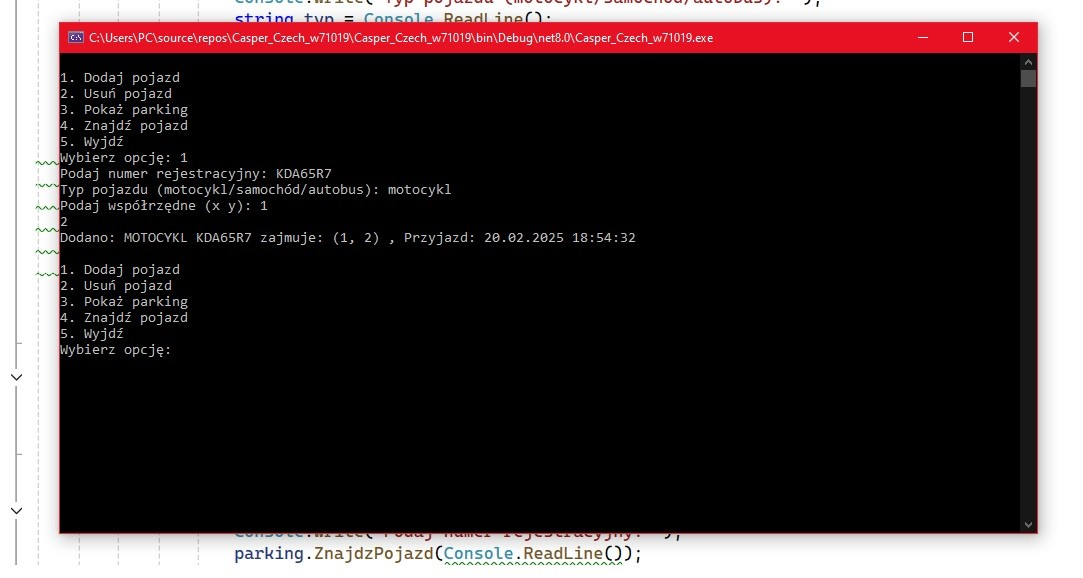
\includegraphics[width=0.8\linewidth]{Dodaj_pojazd.jpg}
    \caption{Dodawanie pojazdu do systemu}
    \label{fig:enter-label}
\end{figure}

\section{Wyświetlanie stanu parkingu}
Aplikacja umożliwia wizualizację aktualnego stanu parkingu, przedstawiając zajęte i wolne miejsca. Użytkownik może w łatwy sposób sprawdzić, które miejsca są dostępne.


\begin{figure}[H]
    \centering
    \includegraphics[width=0.8\linewidth]{Pokaż_parking.jpg}
    \caption{Widok parkingu w systemie}
    \label{fig:enter-label}
\end{figure}
\section{Usuwanie pojazdu}
Gdy pojazd opuszcza parking, użytkownik może usunąć go z systemu, co automatycznie zwalnia zajmowane miejsce.

\begin{figure}[H]
    \centering
    \includegraphics[width=0.8\linewidth]{Usuń_pojazd.jpg}
    \caption{Usuwanie pojazdu z systemu}
\end{figure}

\section{Wyszukiwanie pojazdu}
W celu szybkiego odnalezienia pojazdu system umożliwia jego wyszukiwanie po numerze rejestracyjnym. 

\begin{figure}[H]
    \centering
    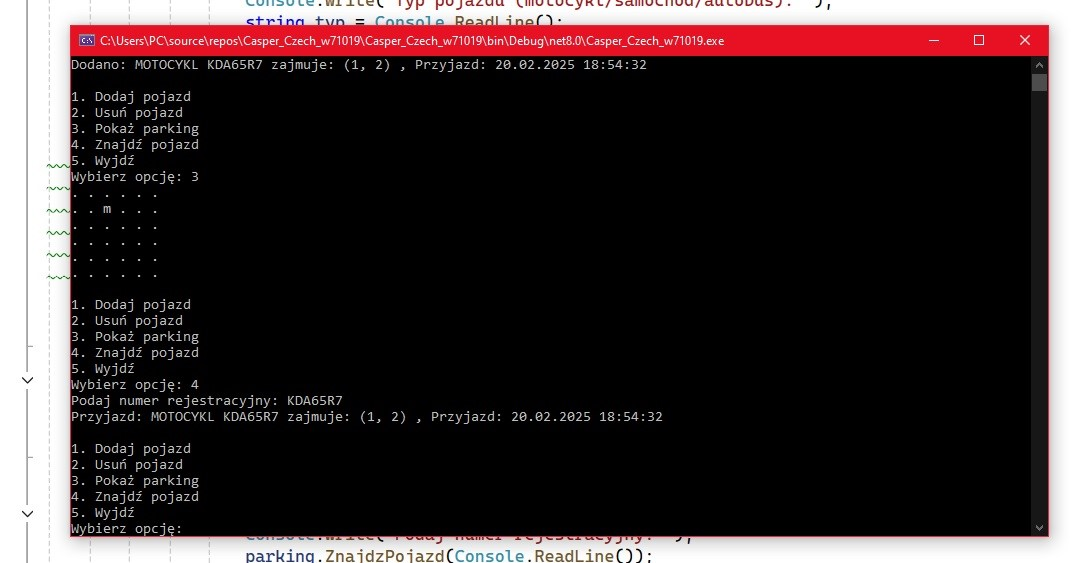
\includegraphics[width=0.8\linewidth]{Znajdz_pojazd.jpg}
    \caption{Wyszukiwanie pojazdu}
\end{figure}

\section{Zamykanie aplikacji}
Użytkownik ma możliwość zamknięcia aplikacji poprzez odpowiednią opcję w menu.

\begin{figure}[H]
    \centering
    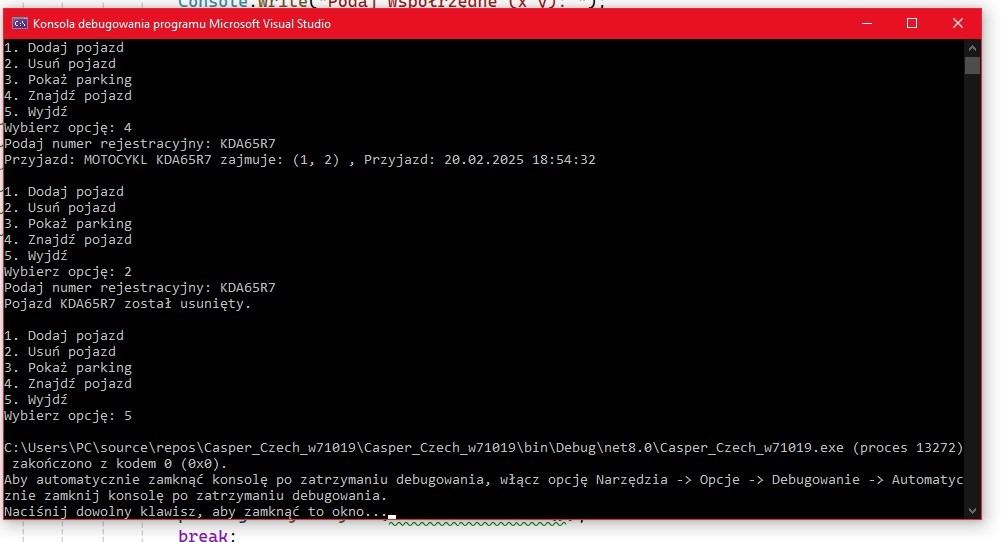
\includegraphics[width=0.8\linewidth]{Wyjdz.jpg}
    \caption{Zamykanie aplikacji}
\end{figure}





% ********** Koniec rozdziału **********
